% Backup D2: what a truncation actually does, for someone who has not seen one.
% (a) cut one bond of the chain; (b) the SVD across that cut ranks the directions
% by weight; (c) keep the largest chi, discard the tail. Circles = state tensors,
% matching the main deck.
\documentclass[tikz,border=3pt]{standalone}
\usepackage{amsmath,amssymb}
\usetikzlibrary{arrows.meta}
\definecolor{tnbulk}{RGB}{86,196,229}
\definecolor{tnbnd}{RGB}{196,98,22}
\definecolor{ink}{RGB}{35,44,58}
\definecolor{warn}{RGB}{176,58,46}
\definecolor{keep}{RGB}{17,122,101}
\begin{document}
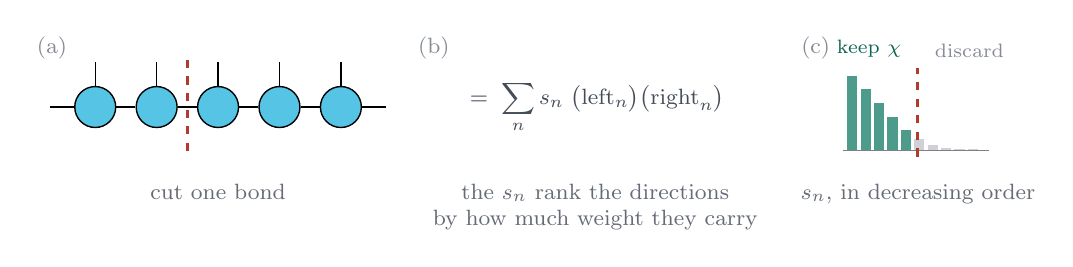
\begin{tikzpicture}[
    W/.style={circle, draw=black, fill=tnbulk, line width=0.5pt,
              minimum size=5.2mm, inner sep=0pt},
    leg/.style={draw=black, line width=0.5pt},
    lab/.style={font=\footnotesize, color=ink!85},
    capt/.style={font=\footnotesize, color=ink!70, align=center},
    pan/.style={font=\footnotesize, color=ink!55}]
  \def\dx{0.78}

  % ---------- (a) cut one bond --------------------------------------------
  \node[pan] at (-0.55,1.30) {(a)};
  \foreach \i in {0,...,4} { \node[W] (a\i) at ({\i*\dx},0.55) {}; }
  \foreach \i/\j in {0/1,1/2,2/3,3/4} { \draw[leg] (a\i.east) -- (a\j.west); }
  \draw[leg] (a0.west) -- ++(-0.30,0);  \draw[leg] (a4.east) -- ++(0.30,0);
  \foreach \i in {0,...,4} { \draw[leg] (a\i.north) -- ++(0,0.30); }
  \draw[warn, dashed, line width=1.0pt] ({1.5*\dx},1.15) -- ({1.5*\dx},-0.05);
  \node[capt, anchor=north] at ({2*\dx},-0.30) {cut one bond};

  % ---------- (b) the SVD across it ----------------------------------------
  \node[pan] at (4.30,1.30) {(b)};
  \node[lab, anchor=west] at (4.55,0.55)
    {$\;=\;\displaystyle\sum_{n} s_n\;\big(\text{left}_n\big)\big(\text{right}_n\big)$};
  \node[capt, anchor=north] at (6.35,-0.30)
    {the $s_n$ rank the directions\\ by how much weight they carry};

  % ---------- (c) keep the largest -----------------------------------------
  \node[pan] at (9.15,1.30) {(c)};
  \foreach \i/\h in {0/0.95,1/0.78,2/0.60,3/0.42,4/0.26,5/0.14,6/0.07,7/0.035,8/0.02,9/0.012} {
    \pgfmathsetmacro\col{\i<5 ? 1 : 0}
    \ifnum\i<5
      \fill[keep!75] ({9.55+\i*0.17},0) rectangle ({9.68+\i*0.17},{\h});
    \else
      \fill[ink!22]  ({9.55+\i*0.17},0) rectangle ({9.68+\i*0.17},{\h});
    \fi }
  \draw[leg, ink!60] (9.50,0) -- (11.35,0);
  \draw[warn, dashed, line width=0.9pt] (10.44,-0.08) -- (10.44,1.05);
  \node[lab, color=keep!80!black, anchor=south east, font=\scriptsize]
    at (10.36,1.06) {keep $\chi$};
  \node[lab, color=ink!55, anchor=south west, font=\scriptsize]
    at (10.54,1.06) {discard};
  \node[capt, anchor=north] at (10.45,-0.30) {$s_n$, in decreasing order};
\end{tikzpicture}
\end{document}
